\chapter{ゲーム理論}

この章では、ランダムな要素を含まない2人用ゲームに焦点を当てます。
そして相手が何をやってもゲームに勝てるような戦略(もしそのような戦略)を見つけることです。
このようなゲームには一般的な戦略があることがわかり、Nimを使ってゲームを分析することができます。
まず、プレイヤーが山から棒を取り除く簡単なゲームを分析し、その後に一般化を行います。

\section{ゲームの状態 - Game states}

最初に$n$本の棒があるゲームを考えます。
プレイヤー$A$と$B$は交互に交代します。最初はプレイヤーAからスタートします。
各手番で1本、2本、3本の棒を山から取り除き、最後の棒を取り除いたプレーヤーがゲームに勝つとします。
n=10の場合、次のようにゲームを進めることができます。

For example, if $n=10$, the game may proceed as follows:
\begin{itemize}[noitemsep]
\item プレイヤーAは2本取る(残り8本)
\item プレイヤーBは3本取る(残り5本)
\item プレイヤーAは1本取る(残り4本)
\item プレイヤーBは2本取る(残り2本)
\item プレイヤーAは2本取って勝ち
\end{itemize}

このゲームは$0,1,2,\ldots,n$の状態からなり、
状態の数は残っているスティックの数に対応します。

\subsubsection{勝ち状態と負け状態 - Winning and losing states}

\index{勝ち状態 - winning state}
\index{負け状態 - losing state}

\key{勝利状態} とは適切に動けば必ず勝ちが確定する状態です。
\key{敗北状態} とは相手が最適なプレイをすればゲームに負ける状態である。
このように、ゲームの状態をすべて分類することで、それぞれの状態が「勝ちの状態」と「負けの状態」のどちらかになることがわかります。

上のゲームを考えます。
状態0は明らかに負け状態で、プレイヤーは何も手を打てません。
状態1、2、3は、最後の1つを取れるので勝ちの状態です。
状態4は逆にどの手を打っても相手が勝ち状態になるため、負け状態と言えます。
一般的には、現在の状態から負け状態にできる現在の状態は勝ち状態であり、
そうでなければ、現在の状態は負け状態である。
これを を利用して、可能な手がない負け状態から始まるゲームのすべての状態を分類 することができます。

状態 $0 \ldots 15$を分類します(Wは勝ち状態、Lは負け状態)。

\begin{center}
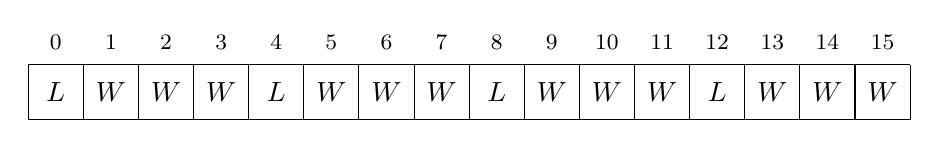
\begin{tikzpicture}[scale=0.7]
\draw (0,0) grid (16,1);

\node at (0.5,0.5) {$L$};
\node at (1.5,0.5) {$W$};
\node at (2.5,0.5) {$W$};
\node at (3.5,0.5) {$W$};
\node at (4.5,0.5) {$L$};
\node at (5.5,0.5) {$W$};
\node at (6.5,0.5) {$W$};
\node at (7.5,0.5) {$W$};
\node at (8.5,0.5) {$L$};
\node at (9.5,0.5) {$W$};
\node at (10.5,0.5) {$W$};
\node at (11.5,0.5) {$W$};
\node at (12.5,0.5) {$L$};
\node at (13.5,0.5) {$W$};
\node at (14.5,0.5) {$W$};
\node at (15.5,0.5) {$W$};

\footnotesize
\node at (0.5,1.4) {$0$};
\node at (1.5,1.4) {$1$};
\node at (2.5,1.4) {$2$};
\node at (3.5,1.4) {$3$};
\node at (4.5,1.4) {$4$};
\node at (5.5,1.4) {$5$};
\node at (6.5,1.4) {$6$};
\node at (7.5,1.4) {$7$};
\node at (8.5,1.4) {$8$};
\node at (9.5,1.4) {$9$};
\node at (10.5,1.4) {$10$};
\node at (11.5,1.4) {$11$};
\node at (12.5,1.4) {$12$};
\node at (13.5,1.4) {$13$};
\node at (14.5,1.4) {$14$};
\node at (15.5,1.4) {$15$};
\end{tikzpicture}
\end{center}

このゲームは簡単で、
$k$が4で割り切れる場合は負け。それ以外は勝ち状態です。
このゲームの最適なプレイ方法は、スティックが4で割り切れる状態にすれば良いです。
もちろん、こちらが動くときに棒の数が4で割り切れないことが条件です。
もし4で割り切れるなら、相手が最適な手を打つ限り勝てません。

\subsubsection{状態グラフ - State graph}

ここで,別のゲームを考えます。
各状態 $k$ において,$x$ が $k$ より小さく $k$ を割り切れる $x$ 本の棒を取り除けるとします。
例えば,状態8では1本,2本,4本の棒を取り除くことができるが、状態7では1本の棒を取り除くことだけが許されるとします。


次の図は、状態$1 \ldots 9$を状態グラフで表したもので、ノードが状態、エッジが取りうる移動です。

\begin{center}
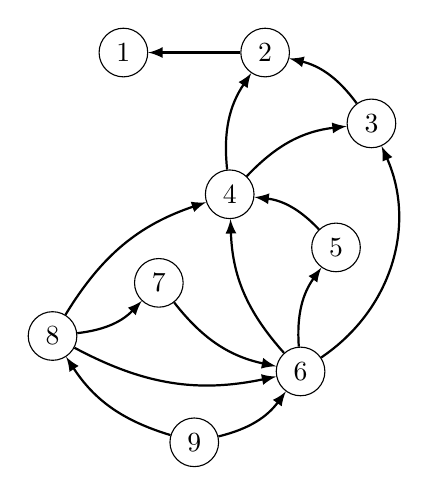
\begin{tikzpicture}[scale=0.9]
\node[draw, circle] (1) at (0,0) {$1$};
\node[draw, circle] (2) at (2,0) {$2$};
\node[draw, circle] (3) at (3.5,-1) {$3$};
\node[draw, circle] (4) at (1.5,-2) {$4$};
\node[draw, circle] (5) at (3,-2.75) {$5$};
\node[draw, circle] (6) at (2.5,-4.5) {$6$};
\node[draw, circle] (7) at (0.5,-3.25) {$7$};
\node[draw, circle] (8) at (-1,-4) {$8$};
\node[draw, circle] (9) at (1,-5.5) {$9$};

\path[draw,thick,->,>=latex] (2) -- (1);
\path[draw,thick,->,>=latex] (3) edge [bend right=20] (2);
\path[draw,thick,->,>=latex] (4) edge [bend left=20] (2);
\path[draw,thick,->,>=latex] (4) edge [bend left=20] (3);
\path[draw,thick,->,>=latex] (5) edge [bend right=20] (4);
\path[draw,thick,->,>=latex] (6) edge [bend left=20] (5);
\path[draw,thick,->,>=latex] (6) edge [bend left=20] (4);
\path[draw,thick,->,>=latex] (6) edge [bend right=40] (3);
\path[draw,thick,->,>=latex] (7) edge [bend right=20] (6);
\path[draw,thick,->,>=latex] (8) edge [bend right=20] (7);
\path[draw,thick,->,>=latex] (8) edge [bend right=20] (6);
\path[draw,thick,->,>=latex] (8) edge [bend left=20] (4);
\path[draw,thick,->,>=latex] (9) edge [bend left=20] (8);
\path[draw,thick,->,>=latex] (9) edge [bend right=20] (6);
\end{tikzpicture}
\end{center}

このゲームの最終状態は常に状態1で、
有効な手がないため負け状態です。
状態$1 \ldots 9$の勝ち状態と負け状態は次のとおりです。

\begin{center}
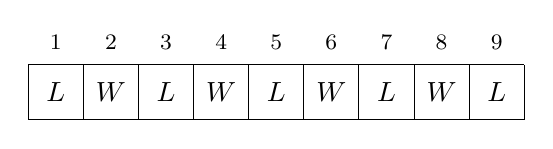
\begin{tikzpicture}[scale=0.7]
\draw (1,0) grid (10,1);

\node at (1.5,0.5) {$L$};
\node at (2.5,0.5) {$W$};
\node at (3.5,0.5) {$L$};
\node at (4.5,0.5) {$W$};
\node at (5.5,0.5) {$L$};
\node at (6.5,0.5) {$W$};
\node at (7.5,0.5) {$L$};
\node at (8.5,0.5) {$W$};
\node at (9.5,0.5) {$L$};

\footnotesize
\node at (1.5,1.4) {$1$};
\node at (2.5,1.4) {$2$};
\node at (3.5,1.4) {$3$};
\node at (4.5,1.4) {$4$};
\node at (5.5,1.4) {$5$};
\node at (6.5,1.4) {$6$};
\node at (7.5,1.4) {$7$};
\node at (8.5,1.4) {$8$};
\node at (9.5,1.4) {$9$};
\end{tikzpicture}
\end{center}

意外かもしれませんがこのゲームは、偶数の時勝ち状態で、奇数の時負け状態です。

\section{Nim - Nim game}

\index{Nim - nim game}

\key{Nim - nim game}は単純なゲームですが同じ戦略を用いて他の多くのゲームを行 うことができるため、
ゲーム理論において重要な考え方です。

nimには$n$個の山があり、各山にはある数の棒があります。
プレイヤーは交互に移動し、まだ棒が入っている山を選び、そこから 任意の本数の棒を取り除きます。
最後のスティックを取り除いたプレイヤーが勝者です。

nimの初期状態は$[x_1,x_2,\ldots,x_n]$で与えられ、
$x_k$ は$k$個目の山のスティックの数とします。
例えば,$[10, 12, 5]$ は10,12,5のスティックを持つ三つの山がある初期状態です。
$[0,0,\ldots,0]$の状態は,棒を1本も取り出せないので負け状態であり,これが常に最終状態です。

\subsubsection{考察 - Analysis}

\index{nim sum}
nim sum $s$を用いて分析を行うことができます\footnote{The optimal strategy
for nim was published in 1901 by C. L. Bouton \cite{bou01}.}。
$s = x_1 \oplus x_2 \oplus \cdots \oplus x_n$として$\oplus$はXOR演算です。
$s$が0の時は負けでそれ以外は勝ち状態です。
例えば$[10,12,5]$は$10 \oplus 12 \oplus 5 = 3$なので勝ち状態です。

ですがnim sumとnimゲームはどのように関係しているのでしょうか?
nimの状態が変化したときに、nim sumがどのように変化するかを見ていいます。
最終状態 $[0,0,\ldots,0]$ は負け状態で、その$s$は0です。
他の負け状態を考えるとどのような動きも勝ち状態になります。
なぜなら、一つの値$x_k$が変化すると、nim sumも変化するので、どんな作業の後もnim sumは0と異なるからです。

勝ち組の状態を考えます。$x_k \oplus s < x_k$となる山$k$があれば,負け状態に遷移できます。つまり勝てます。
この場合,山$k$からスティックを取り除き,$x_k \oplus s$のスティックを含むようにすれば,負け状態に移行できます。
このような山は必ず存在し、いずれかの$x_k$ は s の 左端の1ビットの1ビットを持った数です。

$[10, 12, 5]$の状態を考えてみましょう。
この状態はnim sumが3なので勝ちの状態であり、そのような 手を見つけます。

\begin{center}
\begin{tabular}{r|r}
10 & \texttt{1010} \\
12 & \texttt{1100} \\
5 & \texttt{0101} \\
\hline
3 & \texttt{0011} \\
\end{tabular}
\end{center}

この場合、10本ある山がnim sumの左端の1ビットの位置に1ビットを持つ唯一の山です。

\begin{center}
\begin{tabular}{r|r}
10 & \texttt{10\underline{1}0} \\
12 & \texttt{1100} \\
5 & \texttt{0101} \\
\hline
3 & \texttt{00\underline{1}1} \\
\end{tabular}
\end{center}

山の本数は $10 \oplus 3 = 9$にしたいので1本だけ取ります。
この後、状態は$[9, 12, 5]$となり、負け状態に遷移できます。

\begin{center}
\begin{tabular}{r|r}
9 & \texttt{1001} \\
12 & \texttt{1100} \\
5 & \texttt{0101} \\
\hline
0 & \texttt{0000} \\
\end{tabular}
\end{center}

\subsubsection{misere nim game - Misère game}

\index{misère game}

\key{misere nim game - misère game}はゲームの目的が逆です。
つまり、最後のスティックを取ったプレイヤーがゲームに負けます。
misere nim gameは標準のnimとほぼ同じ様に考えられます。

最初は標準的なnimゲームのようを行うが、ゲームの終盤に戦略を変えます。
戦略を変えるのは、次の手の後に各山が最大で1本の棒を含むような状況で導入されることになる。

オリジナルのゲームでは、1本の棒を持つヒープが偶数個になるような手を選ぶべきです。
しかし、misèreゲームでは、1本の棒で奇数個の山ができるようにします。

まず、この戦略が変化する状態が必ずゲームに現れます。
この状態になったとき、ちょうど複数のスティックを持つ山が一つ含まれているので、
ニムサムは0ではないので、勝利が確定します。

\section{Sprague–Grundy theorem}

\index{Sprague–Grundy theorem}

The \key{Sprague–Grundy theorem}\footnote{The theorem was
independently discovered by R. Sprague \cite{spr35} and P. M. Grundy \cite{gru39}.} generalizes the
strategy used in nim to all games that fulfil
the following requirements:

\begin{itemize}[noitemsep]
\item There are two players who move alternately.
\item The game consists of states, and the possible moves
in a state do not depend on whose turn it is.
\item The game ends when a player cannot make a move.
\item The game surely ends sooner or later.
\item The players have complete information about
the states and allowed moves, and there is no randomness in the game.
\end{itemize}
The idea is to calculate for each game state
a Grundy number that corresponds to the number of
sticks in a nim heap.
When we know the Grundy numbers of all states,
we can play the game like the nim game.

\subsubsection{Grundy numbers}

\index{Grundy number}
\index{mex function}

The \key{Grundy number} of a game state is
\[\textrm{mex}(\{g_1,g_2,\ldots,g_n\}),\]
where $g_1,g_2,\ldots,g_n$ are the Grundy numbers of the
states to which we can move,
and the mex function gives the smallest
nonnegative number that is not in the set.
For example, $\textrm{mex}(\{0,1,3\})=2$.
If there are no possible moves in a state,
its Grundy number is 0, because
$\textrm{mex}(\emptyset)=0$.

For example, in the state graph
\begin{center}
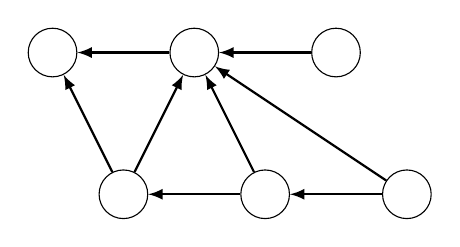
\begin{tikzpicture}[scale=0.9]
\node[draw, circle] (1) at (0,0) {\phantom{0}};
\node[draw, circle] (2) at (2,0) {\phantom{0}};
\node[draw, circle] (3) at (4,0) {\phantom{0}};
\node[draw, circle] (4) at (1,-2) {\phantom{0}};
\node[draw, circle] (5) at (3,-2) {\phantom{0}};
\node[draw, circle] (6) at (5,-2) {\phantom{0}};

\path[draw,thick,->,>=latex] (2) -- (1);
\path[draw,thick,->,>=latex] (3) -- (2);
\path[draw,thick,->,>=latex] (5) -- (4);
\path[draw,thick,->,>=latex] (6) -- (5);
\path[draw,thick,->,>=latex] (4) -- (1);
\path[draw,thick,->,>=latex] (4) -- (2);
\path[draw,thick,->,>=latex] (5) -- (2);
\path[draw,thick,->,>=latex] (6) -- (2);
\end{tikzpicture}
\end{center}
the Grundy numbers are as follows:
\begin{center}
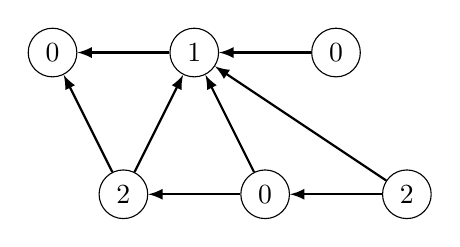
\begin{tikzpicture}[scale=0.9]
\node[draw, circle] (1) at (0,0) {0};
\node[draw, circle] (2) at (2,0) {1};
\node[draw, circle] (3) at (4,0) {0};
\node[draw, circle] (4) at (1,-2) {2};
\node[draw, circle] (5) at (3,-2) {0};
\node[draw, circle] (6) at (5,-2) {2};

\path[draw,thick,->,>=latex] (2) -- (1);
\path[draw,thick,->,>=latex] (3) -- (2);
\path[draw,thick,->,>=latex] (5) -- (4);
\path[draw,thick,->,>=latex] (6) -- (5);
\path[draw,thick,->,>=latex] (4) -- (1);
\path[draw,thick,->,>=latex] (4) -- (2);
\path[draw,thick,->,>=latex] (5) -- (2);
\path[draw,thick,->,>=latex] (6) -- (2);
\end{tikzpicture}
\end{center}
The Grundy number of a losing state is 0,
and the Grundy number of a winning state is
a positive number.

The Grundy number of a state corresponds to
the number of sticks in a nim heap.
If the Grundy number is 0, we can only move to
states whose Grundy numbers are positive,
and if the Grundy number is $x>0$, we can move
to states whose Grundy numbers include all numbers
$0,1,\ldots,x-1$.

As an example, consider a game where
the players move a figure in a maze.
Each square in the maze is either floor or wall.
On each turn, the player has to move
the figure some number
of steps left or up.
The winner of the game is the player who
makes the last move.

The following picture shows a possible initial state
of the game, where @ denotes the figure and *
denotes a square where it can move.

\begin{center}
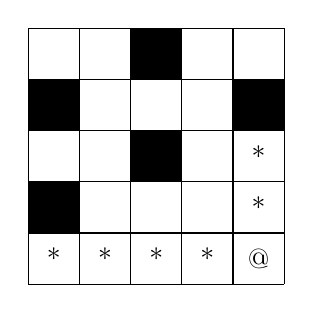
\begin{tikzpicture}[scale=.65]
  \begin{scope}
    \fill [color=black] (0, 1) rectangle (1, 2);
    \fill [color=black] (0, 3) rectangle (1, 4);
    \fill [color=black] (2, 2) rectangle (3, 3);
    \fill [color=black] (2, 4) rectangle (3, 5);
    \fill [color=black] (4, 3) rectangle (5, 4);

    \draw (0, 0) grid (5, 5);

    \node at (4.5,0.5) {@};
    \node at (3.5,0.5) {*};
    \node at (2.5,0.5) {*};
    \node at (1.5,0.5) {*};
    \node at (0.5,0.5) {*};
    \node at (4.5,1.5) {*};
    \node at (4.5,2.5) {*};

  \end{scope}
\end{tikzpicture}
\end{center}

The states of the game are all floor squares
of the maze.
In the above maze, the Grundy numbers
are as follows:

\begin{center}
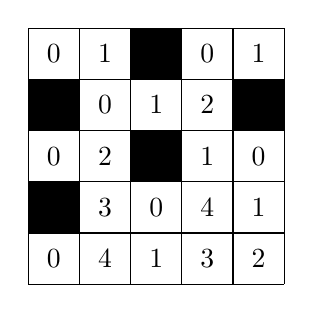
\begin{tikzpicture}[scale=.65]
  \begin{scope}
    \fill [color=black] (0, 1) rectangle (1, 2);
    \fill [color=black] (0, 3) rectangle (1, 4);
    \fill [color=black] (2, 2) rectangle (3, 3);
    \fill [color=black] (2, 4) rectangle (3, 5);
    \fill [color=black] (4, 3) rectangle (5, 4);

    \draw (0, 0) grid (5, 5);

    \node at (0.5,4.5) {0};
    \node at (1.5,4.5) {1};
    \node at (2.5,4.5) {};
    \node at (3.5,4.5) {0};
    \node at (4.5,4.5) {1};

    \node at (0.5,3.5) {};
    \node at (1.5,3.5) {0};
    \node at (2.5,3.5) {1};
    \node at (3.5,3.5) {2};
    \node at (4.5,3.5) {};

    \node at (0.5,2.5) {0};
    \node at (1.5,2.5) {2};
    \node at (2.5,2.5) {};
    \node at (3.5,2.5) {1};
    \node at (4.5,2.5) {0};

    \node at (0.5,1.5) {};
    \node at (1.5,1.5) {3};
    \node at (2.5,1.5) {0};
    \node at (3.5,1.5) {4};
    \node at (4.5,1.5) {1};

    \node at (0.5,0.5) {0};
    \node at (1.5,0.5) {4};
    \node at (2.5,0.5) {1};
    \node at (3.5,0.5) {3};
    \node at (4.5,0.5) {2};
  \end{scope}
\end{tikzpicture}
\end{center}

Thus, each state of the maze game
corresponds to a heap in the nim game.
For example, the Grundy number for
the lower-right square is 2,
so it is a winning state.
We can reach a losing state and
win the game by moving
either four steps left or
two steps up.

Note that unlike in the original nim game,
it may be possible to move to a state whose
Grundy number is larger than the Grundy number
of the current state.
However, the opponent can always choose a move
that cancels such a move, so it is not possible
to escape from a losing state.

\subsubsection{Subgames}

Next we will assume that our game consists
of subgames, and on each turn, the player
first chooses a subgame and then a move in the subgame.
The game ends when it is not possible to make any move
in any subgame.

In this case, the Grundy number of a game
is the nim sum of the Grundy numbers of the subgames.
The game can be played like a nim game by calculating
all Grundy numbers for subgames and then their nim sum.

As an example, consider a game that consists
of three mazes.
In this game, on each turn, the player chooses one
of the mazes and then moves the figure in the maze.
Assume that the initial state of the game is as follows:

\begin{center}
\begin{tabular}{ccc}
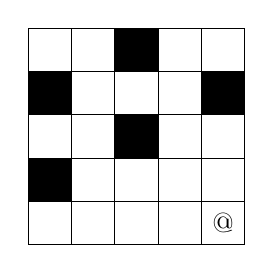
\begin{tikzpicture}[scale=.55]
  \begin{scope}
    \fill [color=black] (0, 1) rectangle (1, 2);
    \fill [color=black] (0, 3) rectangle (1, 4);
    \fill [color=black] (2, 2) rectangle (3, 3);
    \fill [color=black] (2, 4) rectangle (3, 5);
    \fill [color=black] (4, 3) rectangle (5, 4);

    \draw (0, 0) grid (5, 5);

    \node at (4.5,0.5) {@};

    \end{scope}
\end{tikzpicture}
&
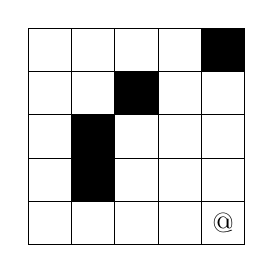
\begin{tikzpicture}[scale=.55]
  \begin{scope}
    \fill [color=black] (1, 1) rectangle (2, 3);
    \fill [color=black] (2, 3) rectangle (3, 4);
    \fill [color=black] (4, 4) rectangle (5, 5);

    \draw (0, 0) grid (5, 5);

    \node at (4.5,0.5) {@};

  \end{scope}
\end{tikzpicture}
&
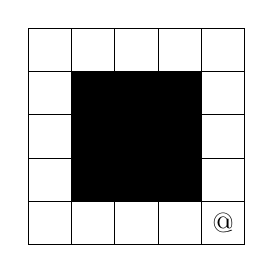
\begin{tikzpicture}[scale=.55]
  \begin{scope}
    \fill [color=black] (1, 1) rectangle (4, 4);

    \draw (0, 0) grid (5, 5);

    \node at (4.5,0.5) {@};
  \end{scope}
\end{tikzpicture}
\end{tabular}
\end{center}

The Grundy numbers for the mazes are as follows:

\begin{center}
\begin{tabular}{ccc}
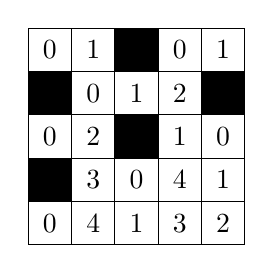
\begin{tikzpicture}[scale=.55]
  \begin{scope}
    \fill [color=black] (0, 1) rectangle (1, 2);
    \fill [color=black] (0, 3) rectangle (1, 4);
    \fill [color=black] (2, 2) rectangle (3, 3);
    \fill [color=black] (2, 4) rectangle (3, 5);
    \fill [color=black] (4, 3) rectangle (5, 4);

    \draw (0, 0) grid (5, 5);

    \node at (0.5,4.5) {0};
    \node at (1.5,4.5) {1};
    \node at (2.5,4.5) {};
    \node at (3.5,4.5) {0};
    \node at (4.5,4.5) {1};

    \node at (0.5,3.5) {};
    \node at (1.5,3.5) {0};
    \node at (2.5,3.5) {1};
    \node at (3.5,3.5) {2};
    \node at (4.5,3.5) {};

    \node at (0.5,2.5) {0};
    \node at (1.5,2.5) {2};
    \node at (2.5,2.5) {};
    \node at (3.5,2.5) {1};
    \node at (4.5,2.5) {0};

    \node at (0.5,1.5) {};
    \node at (1.5,1.5) {3};
    \node at (2.5,1.5) {0};
    \node at (3.5,1.5) {4};
    \node at (4.5,1.5) {1};

    \node at (0.5,0.5) {0};
    \node at (1.5,0.5) {4};
    \node at (2.5,0.5) {1};
    \node at (3.5,0.5) {3};
    \node at (4.5,0.5) {2};
    \end{scope}
\end{tikzpicture}
&
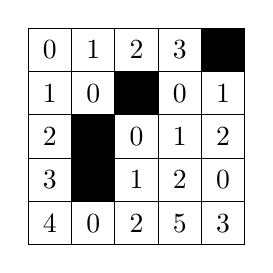
\begin{tikzpicture}[scale=.55]
  \begin{scope}
    \fill [color=black] (1, 1) rectangle (2, 3);
    \fill [color=black] (2, 3) rectangle (3, 4);
    \fill [color=black] (4, 4) rectangle (5, 5);

    \draw (0, 0) grid (5, 5);

    \node at (0.5,4.5) {0};
    \node at (1.5,4.5) {1};
    \node at (2.5,4.5) {2};
    \node at (3.5,4.5) {3};
    \node at (4.5,4.5) {};

    \node at (0.5,3.5) {1};
    \node at (1.5,3.5) {0};
    \node at (2.5,3.5) {};
    \node at (3.5,3.5) {0};
    \node at (4.5,3.5) {1};

    \node at (0.5,2.5) {2};
    \node at (1.5,2.5) {};
    \node at (2.5,2.5) {0};
    \node at (3.5,2.5) {1};
    \node at (4.5,2.5) {2};

    \node at (0.5,1.5) {3};
    \node at (1.5,1.5) {};
    \node at (2.5,1.5) {1};
    \node at (3.5,1.5) {2};
    \node at (4.5,1.5) {0};

    \node at (0.5,0.5) {4};
    \node at (1.5,0.5) {0};
    \node at (2.5,0.5) {2};
    \node at (3.5,0.5) {5};
    \node at (4.5,0.5) {3};
  \end{scope}
\end{tikzpicture}
&
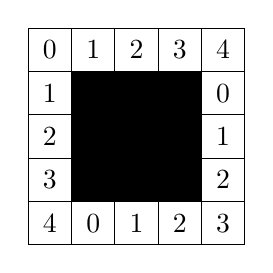
\begin{tikzpicture}[scale=.55]
  \begin{scope}
    \fill [color=black] (1, 1) rectangle (4, 4);

    \draw (0, 0) grid (5, 5);

    \node at (0.5,4.5) {0};
    \node at (1.5,4.5) {1};
    \node at (2.5,4.5) {2};
    \node at (3.5,4.5) {3};
    \node at (4.5,4.5) {4};

    \node at (0.5,3.5) {1};
    \node at (1.5,3.5) {};
    \node at (2.5,3.5) {};
    \node at (3.5,3.5) {};
    \node at (4.5,3.5) {0};

    \node at (0.5,2.5) {2};
    \node at (1.5,2.5) {};
    \node at (2.5,2.5) {};
    \node at (3.5,2.5) {};
    \node at (4.5,2.5) {1};

    \node at (0.5,1.5) {3};
    \node at (1.5,1.5) {};
    \node at (2.5,1.5) {};
    \node at (3.5,1.5) {};
    \node at (4.5,1.5) {2};

    \node at (0.5,0.5) {4};
    \node at (1.5,0.5) {0};
    \node at (2.5,0.5) {1};
    \node at (3.5,0.5) {2};
    \node at (4.5,0.5) {3};
  \end{scope}
\end{tikzpicture}
\end{tabular}
\end{center}

In the initial state, the nim sum of the Grundy numbers
is $2 \oplus 3 \oplus 3 = 2$, so
the first player can win the game.
One optimal move is to move two steps up
in the first maze, which produces the nim sum
$0 \oplus 3 \oplus 3 = 0$.

\subsubsection{Grundy's game}

Sometimes a move in a game divides the game
into subgames that are independent of each other.
In this case, the Grundy number of the game is

\[\textrm{mex}(\{g_1, g_2, \ldots, g_n \}),\]
where $n$ is the number of possible moves and
\[g_k = a_{k,1} \oplus a_{k,2} \oplus \ldots \oplus a_{k,m},\]
where move $k$ generates subgames with
Grundy numbers $a_{k,1},a_{k,2},\ldots,a_{k,m}$.

\index{Grundy's game}

An example of such a game is \key{Grundy's game}.
Initially, there is a single heap that contains $n$ sticks.
On each turn, the player chooses a heap and divides
it into two nonempty heaps such that the heaps
are of different size.
The player who makes the last move wins the game.

Let $f(n)$ be the Grundy number of a heap
that contains $n$ sticks.
The Grundy number can be calculated by going
through all ways to divide the heap into
two heaps.
For example, when $n=8$, the possibilities
are $1+7$, $2+6$ and $3+5$, so
\[f(8)=\textrm{mex}(\{f(1) \oplus f(7), f(2) \oplus f(6), f(3) \oplus f(5)\}).\]

In this game, the value of $f(n)$ is based on the values
of $f(1),\ldots,f(n-1)$.
The base cases are $f(1)=f(2)=0$,
because it is not possible to divide the heaps
of 1 and 2 sticks.
The first Grundy numbers are:
\[
\begin{array}{lcl}
f(1) & = & 0 \\
f(2) & = & 0 \\
f(3) & = & 1 \\
f(4) & = & 0 \\
f(5) & = & 2 \\
f(6) & = & 1 \\
f(7) & = & 0 \\
f(8) & = & 2 \\
\end{array}
\]
The Grundy number for $n=8$ is 2,
so it is possible to win the game.
The winning move is to create heaps
$1+7$, because $f(1) \oplus f(7) = 0$.
